%+++++++++++++++++++++++++++++++++++++++++++++++++++++++++++++++
% SUMMARY    : Optimizers & Backpropagation
%            : University of Southern Maine 
%            : @james.quinlan
%            : Nathaniel Serrano, Silas Qualls - Lecture 12
%+++++++++++++++++++++++++++++++++++++++++++++++++++++++++++++++

\section*{Objectives}
\begin{itemize}
    \item Explain key optimization algorithms used in neural networks
    \item Describe RMSProp and its adaptive learning rate mechanism
    \item Outline the Adam optimizer and its momentum + variance components
    \item Review essential calculus concepts for gradient computation
    \item Introduce the chain-rule–based backpropagation algorithm
\end{itemize}

\rule[0.0051in]{\textwidth}{0.00025in}
% ----------------------------------------------------------------
\section{Optimizers}
\subsection{RMSProp}

\begin{itemize}
    \item Root Mean Square Propagation
    \item Proposed by Geoffrey Hinton during a series of Coursera lectures in 2012
\end{itemize}
RMSProp typically has a slow convergence rate, since it oscillates more than it moves left to right.

However, it can be updated differently in different dimensions, meaning we can adjust the rate at which the gradient descent oscillates up/down as it moves left to right

\begin{center}
\begin{tikzpicture}
  \begin{axis}[
    view={0}{90},               % Top-down view
    xlabel={$w_1$},
    ylabel={$w_2$},
    axis lines=middle,
    ticks=none,
    enlargelimits=true,
    title={RMSProp Descent Path on Loss Contours},
    colormap/viridis,
    clip=false
  ]

    % Draw contour lines of elliptical bowl: z = w1^2 + 4w2^2
    \addplot3[
      contour gnuplot={
        levels={1, 2, 4, 8, 16},
        draw color=black,
      },
      thick,
      domain=-3:3,
      domain y=-3:3,
    ]
    {x^2 + 4*y^2};

    % Add RMSProp oscillatory descent path (bounces in w2, slow in w1)
    \addplot[
      color=red,
      thick,
      mark=*,
      mark size=1pt
    ] coordinates {
      (-2.5, 0.5)
      (-2.2, 0.8)
      (-1.9, 0.3)
      (-1.6, -0.2)
      (-1.3, -0.4)
      (-1.0, -0.3)
      (-0.7, -0.1)
      (-0.4,  0.05)
      (-0.2,  0.01)
      ( 0.0,  0.0)
    };

  \end{axis}
\end{tikzpicture}
\end{center}


\textbf{Standard:} \[ w =
\begin{bmatrix}
w_1 \\
w_2 \\
\vdots \\
w_n
\end{bmatrix}, \nabla C = \begin{bmatrix}
    \frac{\partial C}{\partial w_1} \\
\frac{\partial C}{\partial w_2} \\
\vdots \\
\frac{\partial C}{\partial w_n}
\end{bmatrix}
\rightarrow
w=w -\alpha\nabla C
\]

We can adjust this equation:
\begin{itemize}
    \item $w_1$ should increase at a faster rate than $w_2$
    \item This allows for faster convergence, with the gradient descent moving left/right more than oscillating up/down
\end{itemize}
\underline{\textbf{How?}}
\begin{itemize}
    \item Scale components \textit{individually}
    \begin{itemize}
        \item Large gradients $\rightarrow$ small step
        \item Small gradients $\rightarrow$ large step
    \end{itemize}
    \item Hadamard Products
    \begin{itemize}
        \item Element-wise multiplication
        \item Example: \\
        \[
        \begin{bmatrix}
            w_1 \\
            w_2
        \end{bmatrix} \odot 
        \begin{bmatrix}
            3 \\
            2
        \end{bmatrix} =
        \begin{bmatrix}
            3w_1 \\
            2w_2
        \end{bmatrix}
        \]
    \end{itemize}
    
\end{itemize}
We can apply element-wise operations to RMSProp's update equations:
\[
v_{t+1} = \beta v_t + (1-\beta) \nabla C(w_2)^2
\]

\[w_{t+1} = w_t - \alpha \frac{\nabla C(w_t)}{\sqrt{v}+\epsilon}\]
\begin{itemize}
    \item $w$ = weights
    \item $v$ = Exponentially decaying average of the squared gradients
    \item $\nabla C (w)^2$ is an element-wise product:
     \[
            \begin{bmatrix}
            C_1 \\
            C_2 \\
            \vdots
        \end{bmatrix} \odot 
        \begin{bmatrix}
            C_1 \\
            C_2 \\
            \vdots
        \end{bmatrix} =
        \begin{bmatrix}
            C_1^2 \\
            C_2^2 \\
            \vdots
        \end{bmatrix}
    \]
    \item $\frac{\nabla C(w_t)}{\sqrt{v}+\epsilon}$ is an elemental-wise division:
\end{itemize}
\[
\frac{\nabla C}{\sqrt{v}} = 
\begin{bmatrix}
    C_1 \\
    C_2 \\
    \vdots \\
    C_n
\end{bmatrix}
\oslash
\begin{bmatrix}
    \sqrt{v_1} \\
    \sqrt{v_2} \\
    \vdots \\
    \sqrt{v_n}
\end{bmatrix}
=
\begin{bmatrix}
    C_1/\sqrt{v_1} \\
    C_2/\sqrt{v_2} \\
    \vdots \\
    C_n/\sqrt{v_n}
\end{bmatrix}
\]
If $v_1$ is large, $C_1/\sqrt{v_1}$ will shrink, making it oscillate less and move more to the right.

$\epsilon \approxeq 10^-8$ typically. This is used to prevent division by $0$ without affecting results in a noticeable way. This process is known as \textbf{numerical stability}.

\subsection{Adam}
\begin{itemize}
    \item Adam = RMSProp + Momentum = ``Adaptive Moments''
    \begin{itemize}
        \item 1st moment = mean (Momentum)
        \item 2nd moment = variance (RMSProp)
    \end{itemize}
    \item Combines the best of both worlds
    \item Works well with almost all architectures
    \begin{itemize}
        \item ANN
        \item CNN
        \item RNN
        \item etc...
    \end{itemize}
\end{itemize}

Adam's update equations:
\[
m_{t+1} = \beta_1 m_t + (1-\beta_1)\nabla C(w) \\
\]
\[
v_{t+1} = \beta_2 v_t+t + (1-\beta_2) \nabla C(w)^2
\]
\begin{itemize}
    \item $C$ = cost $\equiv$ $L$ = loss
    \item m = mean (Momentum)
    \item v = \textbf{variance} (NOT velocity)
\end{itemize}
\[\longrightarrow
w_{t+1} = w_t - \alpha \frac{m_{t+1}}{\sqrt{v_{t+1}}+\epsilon}
\]
With initializations:
\begin{itemize}
    \item v = 0
    \item m = 0
    \item w = 0 (Arbitrarily chosen; can be random)
\end{itemize}
In previous lectures we have seen multiple weight equations with gradients. In Adam, gradients have been bundled into $m$.
\newline
\newline
We can make some slight changes to account for bias:
\[
\hat{m}_{t+1} = \frac{m_{t+1}}{1-\beta_1^t}
\]
\begin{itemize}
    \item at $m_1 \rightarrow 1-\beta_1^1 \neq 0 \approx 0.999...$
\end{itemize}
\[
\hookrightarrow
\hat{v}_{t+1} = \frac{v_{t+1}}{1-\beta_2^t}
\]
\[
\hookrightarrow \boxed{
w_{t+1} = w_t - \alpha \frac{\hat{m}_{t+1}}{\sqrt{\hat{v}_{t+1}}+\epsilon}}
\]
We now have our new bias corrected equation made up of the \textbf{bias-correction terms} $\hat{m}_{t+1}$ and $\hat{v}_{t+1}$
\section{Calculus Review}

\subsection{Differential Calculus}

Differential calculus is concerned with the study of how quantities change. A central theme is understanding how a function changes with respect to its inputs.

\begin{center}
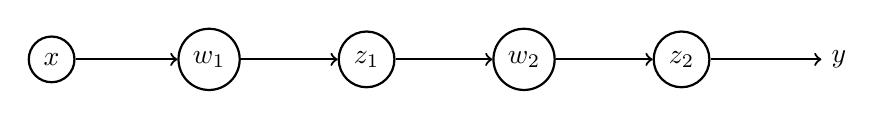
\begin{tikzpicture}[->, thick]
  \node[circle, draw] (x) at (0,0) {$x$};
  \node[circle, draw] (w1) at (2,0) {$w_1$};
  \node[circle, draw] (z1) at (4,0) {$z_1$};
  \node[circle, draw] (w2) at (6,0) {$w_2$};
  \node[circle, draw] (z2) at (8,0) {$z_2$};
  \node (y) at (10,0) {$y$};
  
  \draw (x) -- (w1);
  \draw (w1) -- (z1);
  \draw (z1) -- (w2);
  \draw (w2) -- (z2);
  \draw (z2) -- (y);
\end{tikzpicture}
\end{center}

This diagram represents a simple computational graph. Variables $x$, $w_1$, $w_2$, etc., flow through functions and operations to compute an output $y$. 

\subsection{Goal: Minimize Cost}

We aim to minimize some cost function, such as the squared loss:

\[
\text{Loss} = (y - \hat{y})^2
\]

\subsection{Change and Derivatives}

To achieve this, we need to understand how the output changes with respect to changes in the input — this is captured by the derivative:

\[
\frac{d}{dx}
\]

The derivative tells us how quantities flow and change with respect to one another.

\subsection{Single Variable Case}

In the single variable case, the derivative is:

\[
\frac{dz}{dx}
\]

This helps in understanding how a small change in $x$ affects $z$.    

\subsection{The Chain Rule}

The chain rule is a fundamental rule in differential calculus that allows us to compute the derivative of a composition of functions.

If we have two functions \( f \) and \( g \), then:

\[
(f \circ g)'(x) = f'(g(x)) \cdot g'(x)
\]

This is essential for calculating derivatives when functions are composed (e.g., layers in a neural network).

\subsubsection{Function Composition}

\[
F(x) = f(g(h(x)))
\]

Applying the chain rule:

\[
\frac{dF}{dx} = f'(g(h(x))) \cdot g'(h(x)) \cdot h'(x)
\]

This generalizes to many layers of nested functions.

\subsection{Neural Network Example}

Assume a simple feedforward computation:

\begin{align*}
x &= \text{input} \\
z_1 &= w_1 x \\
z_2 &= w_2 z_1 \\
y &= f(z_2)
\end{align*}

If our loss is based on \( y \), then we want to compute:

\[
\frac{d\mathcal{L}}{dw_2} = \frac{d\mathcal{L}}{dy} \cdot \frac{dy}{dz_2} \cdot \frac{dz_2}{dw_2}
\]

This shows how gradients "flow backward" through the network using the chain rule, which is the core idea behind \textbf{backpropagation}.

\subsection{Example: Applying the Chain Rule to a Composition}

Let:

\[
\mathcal{L} = \mathcal{L}(z^{(4)}) = 3z^{(4)} = 6
\]

Suppose we are interested in computing the derivative with respect to earlier variables using the chain rule.

Assume:

\[
z^{(4)} = a^{(3)} w^{(4)} + b^{(4)}
\]

Then:

\[
\frac{d\mathcal{L}}{dz^{(4)}} = 3, \quad \text{so}
\quad \frac{d\mathcal{L}}{da^{(3)}} = \frac{d\mathcal{L}}{dz^{(4)}} \cdot \frac{dz^{(4)}}{da^{(3)}}
= 3 \cdot w^{(4)}
\]

\subsubsection*{Example Using a Quadratic Function}

If we let:

\[
z^{(4)} = (x - 3)^2
\]

Then:

\[
\frac{d\mathcal{L}}{dx} = \frac{d\mathcal{L}}{dz^{(4)}} \cdot \frac{dz^{(4)}}{dx}
= 3 \cdot 2(x - 3) = 6(x - 3)
\]

\subsection{Backpropagation Flow}

The gradient continues backward layer by layer, following the chain rule. Each step requires computing:

\[
\frac{d\mathcal{L}}{dz^{(l)}} = \frac{d\mathcal{L}}{dz^{(l+1)}} \cdot \frac{dz^{(l+1)}}{dz^{(l)}}
\]

This recursive application forms the core of backpropagation in neural networks.

\bigskip

In the next section, we walk through this process step-by-step using detailed notation and examples.

\subsection{Backpropagation: Chain Rule}

To understand backpropagation, we rely heavily on the chain rule from calculus.

\subsubsection*{Chain Rule (2 Functions)}

\[
(f \circ g)'(x) = f'(g(x)) \cdot g'(x)
\]

For a composition of three functions:

\[
[f \circ g \circ h](x) = f'(g(h(x))) \cdot g'(h(x)) \cdot h'(x)
\]

Using Leibniz notation (derivative of $y$ with respect to $x$):

\[
\frac{dy}{dx} = \frac{dy}{dz} \cdot \frac{dz}{dw} \cdot \frac{dw}{dx}
\]

Alternatively, in Newton notation: $\dot{y}$ denotes the derivative with respect to time.

The chain rule allows us to compute the derivative of composite functions by multiplying the derivatives of the inner functions.

\textbf{Example:} Let $y = \sin(x^2)$, then $\frac{dy}{dx} = \cos(x^2) \cdot 2x$

The chain rule is a key component in backpropagation in neural networks, where gradients are passed backward through layers using this principle.

\subsubsection*{Example Setup}

Let:

\begin{align*}
w_0 &= x \\
w_1 &= h(w_0) \\
w_2 &= g(w_1) \\
w_3 &= f(w_2) = f(g(h(x))) = y
\end{align*}

We are interested in computing:

\[
\frac{dy}{dx}
\]

To do so, we take derivatives step-by-step:

\[
\frac{dy}{dx} = \frac{dy}{dw_2} \cdot \frac{dw_2}{dw_1} \cdot \frac{dw_1}{dx}
\]

\section{Backpropagation Flow}

\subsubsection*{Backpropagation Chain}

In a typical neural network layer:

\[
z^{(l)} = a^{(l-1)} w^{(l)} + b^{(l)}
\]

\[
a^{(l)} = \sigma(z^{(l)})
\]

Where:
- $\sigma$ is an activation function (e.g., sigmoid or ReLU).
- $a^{(l)}$ is the activation at layer $l$.
- $z^{(l)}$ is the linear combination before activation.

\subsubsection*{Gradient Flow}

From the output layer backward, we compute:

\[
\frac{\partial C}{\partial a^{(L)}} = 2(a^{(L)} - y)
\]

\[
\frac{\partial a^{(L)}}{\partial z^{(L)}} = \sigma'(z^{(L)}), \quad \frac{\partial z^{(L)}}{\partial w^{(L)}} = a^{(L-1)}
\]

Using the chain rule:

\[
\frac{\partial C}{\partial w} = \frac{\partial C}{\partial a} \cdot \frac{\partial a}{\partial z} \cdot \frac{\partial z}{\partial w}
\]

This tells us how a small change in a weight affects the overall cost. This is the essence of \textbf{backpropagation}.
